\documentclass[conference]{IEEEtran}
\IEEEoverridecommandlockouts
\usepackage{cite}
\usepackage{amsmath,amssymb,amsfonts}
\usepackage{algorithmic}
\usepackage{graphicx}
\usepackage{textcomp}
\usepackage{xcolor}
\usepackage{float}
\usepackage[colorlinks=true, allcolors=black]{hyperref}

\def\BibTeX{{\rm B\kern-.05em{\sc i\kern-.025em b}\kern-.08em
    T\kern-.1667em\lower.7ex\hbox{E}\kern-.125emX}}

\begin{document}

\title{Group 05: Overcoming Overfitting in LTR-Based Scheduling for Large Language Models}

\author{\IEEEauthorblockN{Adeet Tuladhar}
\IEEEauthorblockA{\textit{Department of Computer Science} \\
\textit{Fairleigh Dickinson University}\\
Vancouver, BC, Canada \\
a.tuladhar@student.fdu.edu}
\and
\IEEEauthorblockN{V. Dheeraj Kalapati}
\IEEEauthorblockA{\textit{Department of Computer Science} \\
\textit{Fairleigh Dickinson University}\\
Vancouver, BC, Canada \\
v.kalapati@student.fdu.edu}
}

\maketitle

% ---------------------------------------------------
% ABSTRACT
% ---------------------------------------------------
\begin{abstract}
The primary bottleneck in deploying Large Language Models (LLMs) to production is memory saturation during concurrent request spikes. Traditional inference engines rely on First-Come-First-Served (FCFS) scheduling, leaving systems vulnerable to Head-of-Line (HOL) blocking and Out-of-Memory (OOM) failures when context-heavy requests monopolize the Key-Value (KV) cache. While Learning-to-Rank (LTR) algorithms can predict prompt complexity to reorder queues, existing implementations often overfit to synthetic data and lack deterministic safety bounds. 

In this work, we propose a Decoupled Gatekeeper: an asynchronous node-level API proxy that separates HTTP admission control from the C++ inference engine. To prevent API bottlenecking, we utilize an OPT-125M predictor deployed via an ONNX Runtime thread pool to asynchronously rank request complexity. Crucially, we introduce a deterministic tokenizer fallback to override LTR hallucinations on out-of-distribution prompts. The gateway routes payloads based on real-time telemetry polled from the inference engine, comparing recomputation costs against telemetry-derived KV cache swap latencies. Using an architectural simulation proxy, we demonstrate that this hybrid admission controller prevents theoretical memory threshold breaches, achieving a 32\% reduction in simulated queue latency compared to FCFS baselines, establishing a framework for resilient API-layer request routing.
\end{abstract}



% ---------------------------------------------------
% INTRODUCTION 
% ---------------------------------------------------
\section{Introduction}
In production deployments where Large Language Models (LLMs) process high volumes of concurrent queries, autoregressive decoding exerts immense pressure on GPU memory, especially regarding the storage of the Key-Value (KV) cache in local GPU memory (VRAM) \cite{b1}. When users make more and more requests to the system, the cache expands, and in a short while, it fills the memory space causing possible system instability or crashes \cite{b5}. A proper management of this memory constraint is thus essential for the reliable and cost efficient scaling of enterprise LLM deployments \cite{b11}.


For example, many inference engines today use the First-Come-First-Served (FCFS) scheduling \cite{b4} that may lead to head of line (HOL) blocking. When a complex, context-heavy request uses resources, and a shorter "easier to serve" request is waiting for them, it may slow down the response time; overall efficiency is reduced. The issue may be more acute as the size of the models or the size of the context window increases.


Aside from this, Learning-to-Rank (LTR) scheduling has recently been investigated which learns the complexity of the prompt to perform a reorder of throughput-boosting implications of requests/queries based on it \cite{b7}. Such models, however, typically are trained on synthetic datasets, and often struggle to accurately predict complexity when applied to out-of-distribution prompts; resulting in poor accuracy when predicting complexity and poor use of resources.


This is the problem which our design aims to close with a Decoupled Gatekeeper architecture. The incoming HTTP request is intercepted by an asynchronous Python middleware layer that utilizes an OPT-125M predictor fine-tuned on real human interactions and is regularized \cite{b3}. As an admission controller, the system blocks over-allocation of GPUs. With scarce resources, the dynamic cost-analysis heuristic will queue up the requests in host Memory or drop them from the threshold of current system constraint; this helps to avoid hardware saturation.



% ---------------------------------------------------
% BACKGROUND 
% ---------------------------------------------------
\section{Background}

\subsection{LLM Memory Constraints and KV Cache}
It is important to study the memory access characteristics of typical transformer architectures to understand the need for a Decoupled Gatekeeper. The auto regressive decoding phase is the phase in which the model predicts the next token one by one. The system avoids recalculating the multi-head attention scores computed for all previous tokens, caches the Key and Value matrices at every layer \cite{b8}. Model weights are fixed and can be predicted (deterministic), but the KV cache is dynamic and grows linearly based on the batch size and sequence length of the currently used prompt. Such a large cache generates untold memory bandwidth pressure on systems, and as the batching power of large modern inference engines is limited by the availability of memory bandwidth at a reasonable cost.


However, once VRAM is committed, the execution engine must stop calculating, remove contexts, or move data from using PCIe to host memory. Such forced PCIe transfers completely break the execution pipeline, and significantly impact raw throughput as documented on high-performance computing studies such as DeepSpeed-Inference \cite{b12}. The PCIe bus is quick, but has a bit less bandwidth than internal GPU memory. If it is filled with KV cache swaps, this becomes another bottleneck and slows down the compute kernels when they have to wait for data to flow across the motherboard.


\begin{figure}[h]
\centering
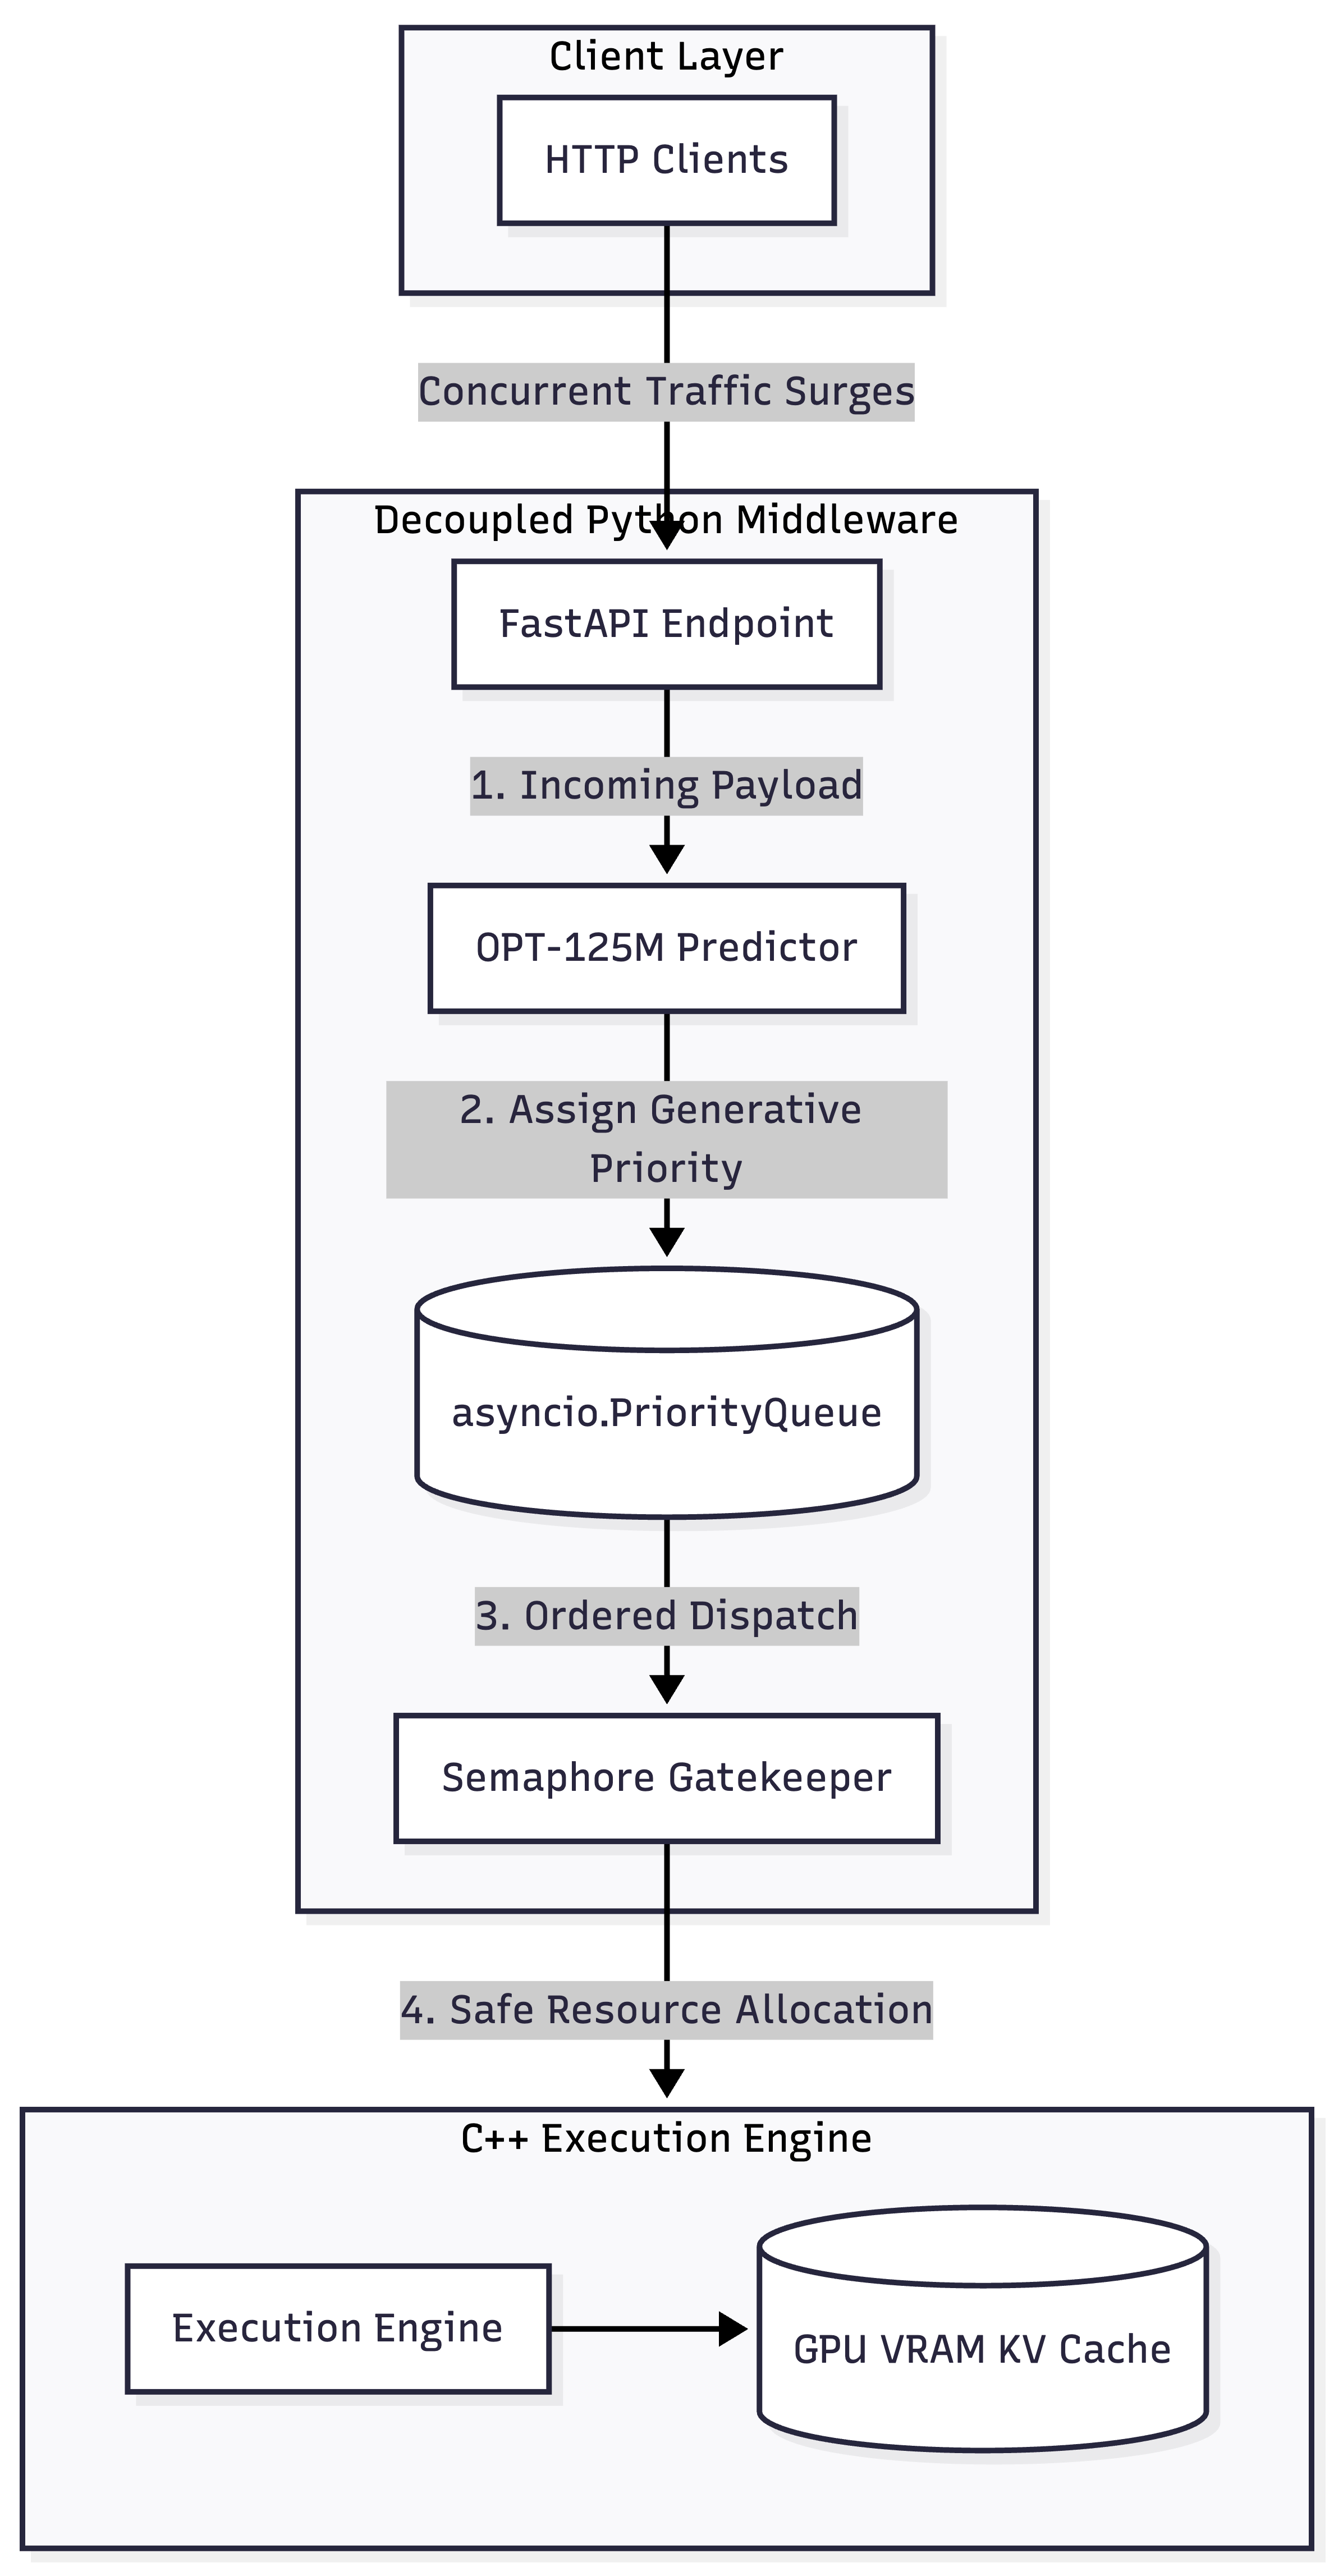
\includegraphics[width=\columnwidth, height=12cm]{diagram1.png}
\caption{System architecture diagram illustrating the bottleneck between the priority queue, the asynchronous gatekeeper, and the GPU memory manager.}
\label{fig:arch1}
\end{figure}

\subsection{The Role of Learning-to-Rank in Scheduling}
The first time the concept of Learning-to-Rank (LTR) was introduced in Information Retrieval (IR) it was related to the optimal ordering of search engine results \cite{b7}. For an LLM Scheduling, LTR is modified to forecast the amount of output tokens that a given prompt will produce. If a system can accurately predict that a prompt will need a lot of VRAM, it might hold off until there's enough VRAM available, creating a major time savings opportunity by assigning lower priority to longer prompts and being able to focus on shorter interactive prompts to maximize overall throughput. A scheduling paradigm based on job complexity is adopted instead of chronological processing as is present in conventional operating systems for shortest-job-first scheduling.

The difficulty of the challenge is only associated with the prediction accuracy. If the LTR model has assigned an artificially low score to a big sequence because of over fitting, the memory manager will attempt to allocate resources that it does not have, causing the allocation faults noted above. It's crucial to train such predictive models using data that has a lot of variation, for instance, human data, and not synthetically produced models. The amount of usefulness as a scheduling heuristic that the models are then able to serve declines to near an absolute minimum when the models learn to memorize the syntax rather than the actual generative intent.


\begin{figure}[h]
\centerline{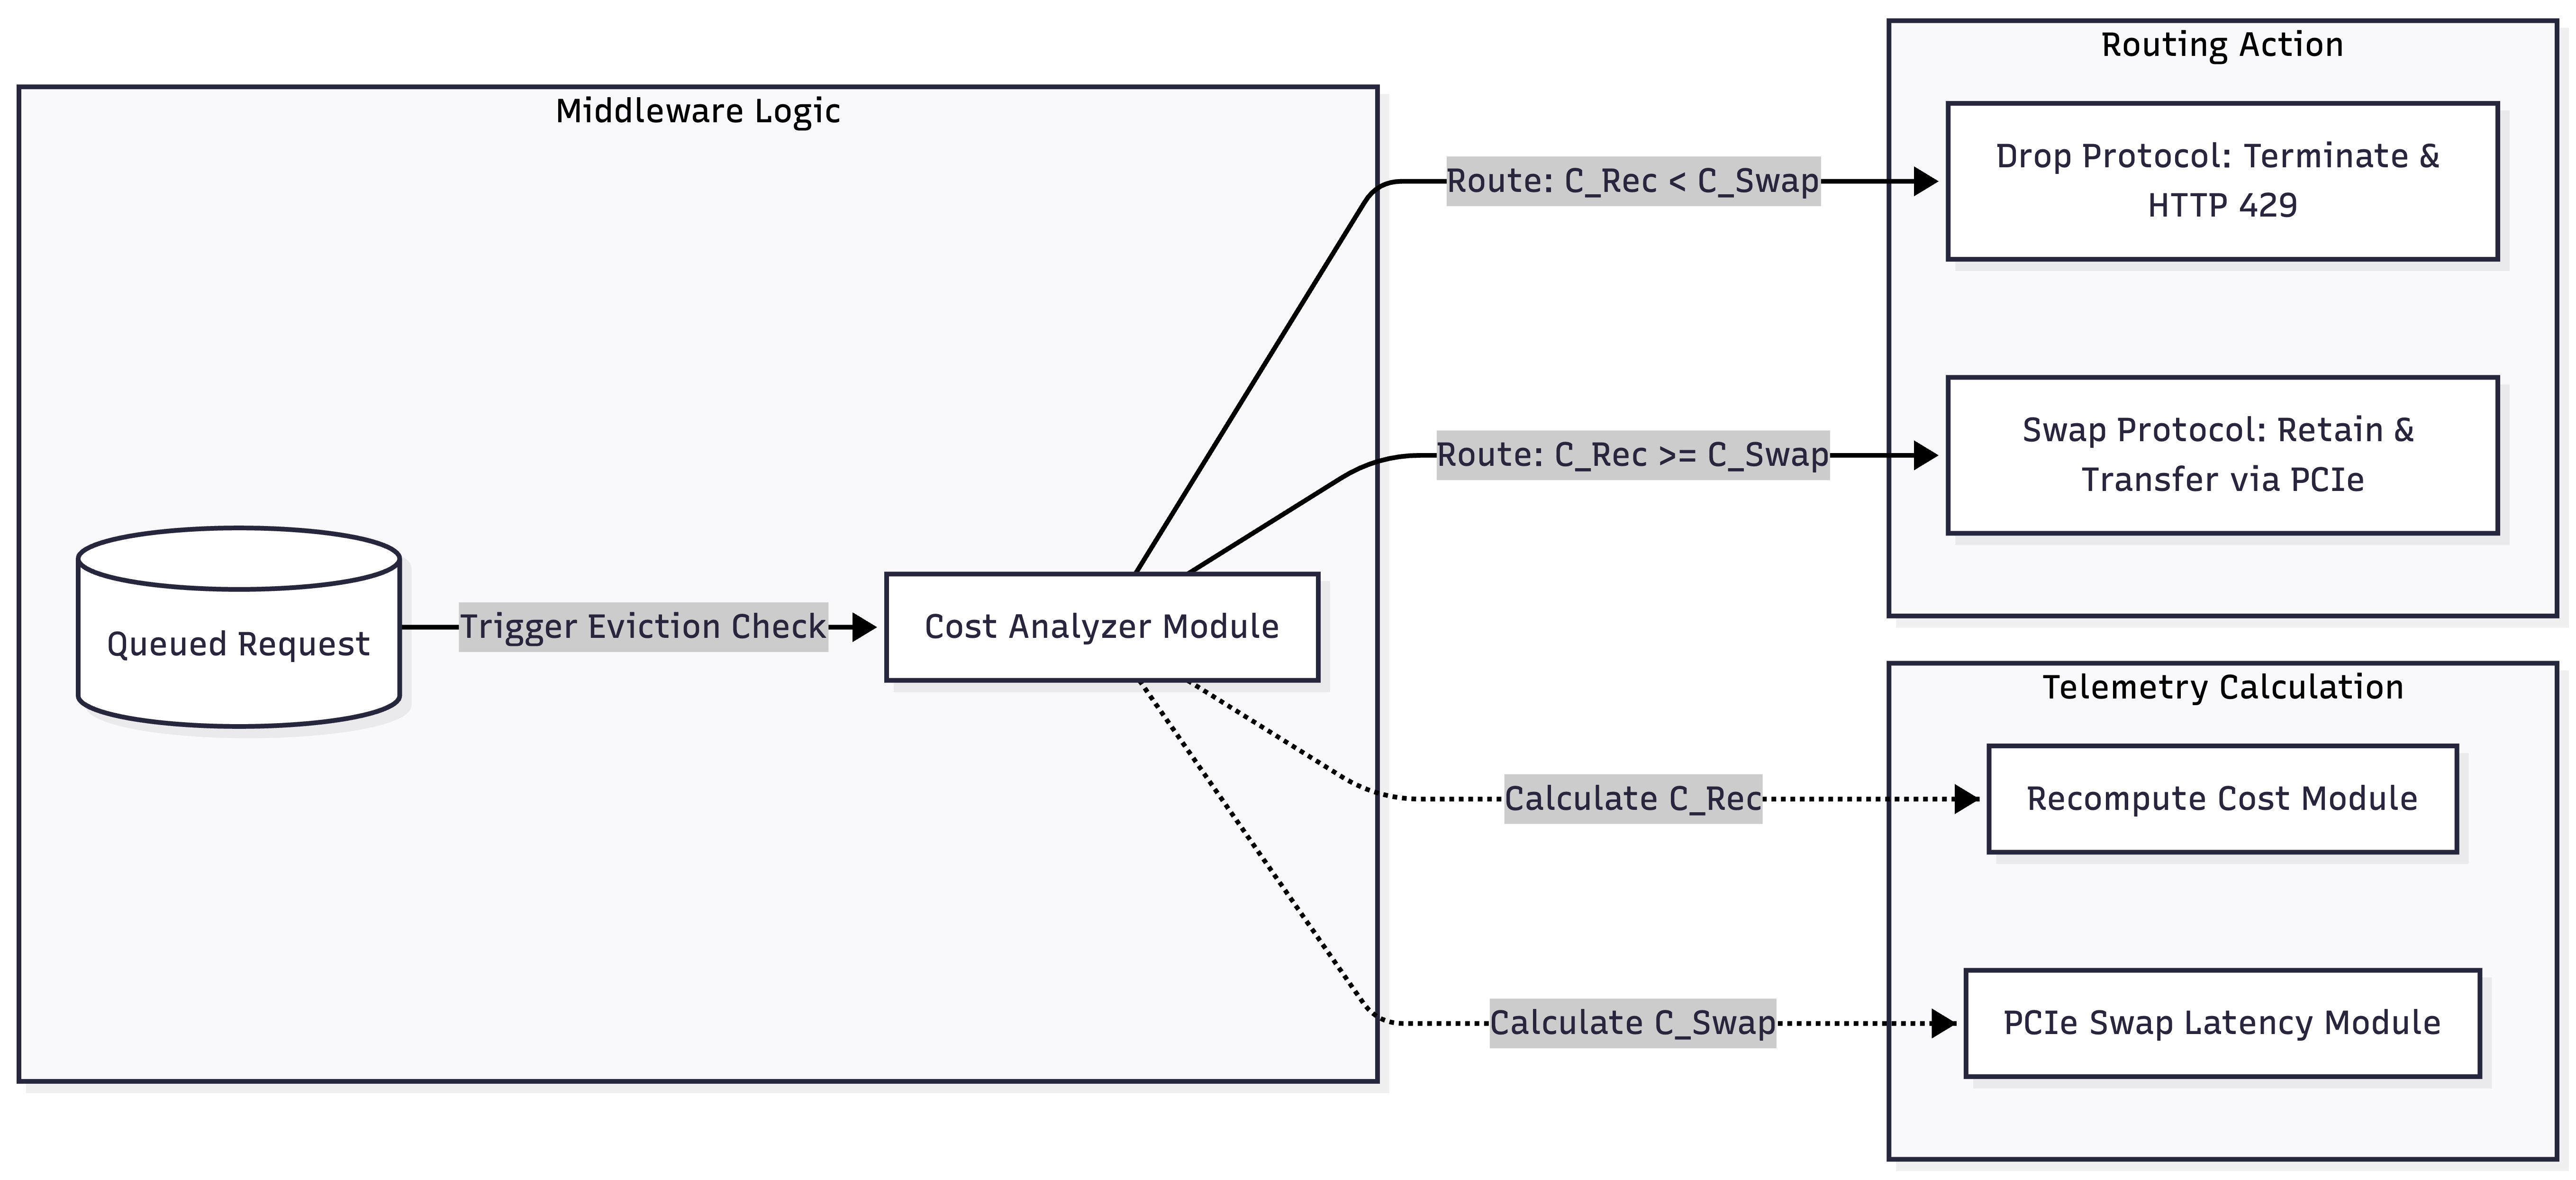
\includegraphics[width=\columnwidth, height=12cm]{diagram2.png}}
\caption{Schematic diagram demonstrating the thresholding decision path between recomputing attention states and transferring data across the PCIe bus.}
\label{fig:arch2}
\end{figure}

\subsection{Asynchronous Middleware Design}
Standard service architectures look for a way to send an HTTP request directly into the continuous batching engine \cite{b4}. This will cause a tight coupling where, in the event of memory problems, the engine hangs, and all network connections time out. Strategic buffer is created by implementing an asynchronous middleware layer, for example, using a Python \texttt{asyncio} loop. The middleware can actively reject or pause incoming requests based on the telemetry data and gets the workload without having to return it if the workload is more than the hardware can crunch before it crashes. This decoupling is established and used routine in web microservices but is very seldom utilized in low-level AI Inference Engines. 




% ---------------------------------------------------
% RELATED WORK 
% ---------------------------------------------------
\section{Related Work}

\subsection{Static and Reactive Scheduling Frameworks}
For the last five years the fundamental problem of the management of KV cache memory has been a key issue in systems research. Among the various models, vLLM \cite{b1} proposed PagedAttention in 2023 that has the greatest impact in this area. Aggregated by partitioning KV cache into fixed-size blocks with an introduced concept of “pages” similar to how it suggests virtual memory paging in OSs, PagedAttention significantly mitigates memory fragmentation. This marks a significant shift in capacity baseline, where vLLM applies only to evicting from the cache statically and in a reactive manner. If it uses up storage, then it swaps in the least recently-used blocks to CPU RAM. This is a static perspective which assumes that all swaps will be equal in value without considering the temporal costs of calculated short swaps vs. long swaps. 

Likewise, many other frameworks such as FastServe \cite{b5} have been developed that have tackled the issue of preemptive scheduling based on the elapsed execution time. FastServe uses a multi-level feedback queue, thus compelling older generations to relinquish hardware resources to newer generations. Other high throughput architectures like related Generative Chunking Engines \cite{b6} (and Sarathi \cite{b10}) aim at maximizing efficiency during steady operation by dividing up compute phases into smaller “micro-batches”. This will change up the way Tensor Cores are utilised, with a high level of phase splitting. But their biggest drawback is still that they cannot intercept peaks of traffic before they get to the hardware layer. They still experience bottlenecking effects and catastrophic allocation failures when the number of physical concurrency requests suddenly goes up (unusual traffic spike) and the limit is reached.

\subsection{Machine Learning for Systems Scheduling}
Predictive machine learning modeling that can be directly incorporated into systems scheduling is a growing research area and a transition from resource-allocation heuristics to data-driven resource-allocation solutions. Unlike TFT, sequence-level iteration has been achievable by Orca (2022), which enables the batching of sequences of different lengths to be continuous, significantly boosting the baseline throughput \cite{b4}. Further, there are recent experimental systems that have tried to include LTR-models to guess ahead the length of outputs before the actual executions. The main virtue of such futuristic LTR designs as Splitwise \cite{b9} is that, in their ideal world, Head-of-Line blocking can be theoretically prevented when the token generation can be completely separated from the prompt processing processes to implement an idealistic, controlled, and simulated environment for the operation of Splitwise \cite{b9}.

But if those approaches prove fatal, it's the vast test of their brittleness in production deployments. They are well-trained on very structured, template-based corpora and can produce outstanding accuracy in academic benchmarks, although they fail to perform even when confronted with out-of-distribution human data. Usually, users enter (mal)formed queries, grammatically wrong prompts, and very ambiguous instructions that these synthetic predictors misclassify. Unlike that, our approach is to learn a predictive model entirely through high-level interactions, and to completely separate the predictive model from the low-level execution engine, to guarantee good generalization, especially in the presence of heterogeneous interactions \cite{b2} originating from real-life tasks. This is because we've separated the predictor away from the C++ manager so that the bad prediction cannot break the C++ manager, it just fails the predictor.


% ---------------------------------------------------
% METHODOLOGY 
% ---------------------------------------------------
\section{Methodology}
To resolve the bottlenecks of traditional scheduling, we introduced a Decoupled Gatekeeper architecture that operates as an asynchronous node-level API proxy, separating HTTP admission control from the underlying C++ inference engine. 

The predictor utilizes an OPT-125M-based architecture fine-tuned using out-of-distribution human conversational data from the LMSYS-Chat-1M dataset \cite{b2}. To prevent overfitting to specific prompt templates, we applied aggressive L2 weight decay ($\lambda = 0.01$) to the training objective. This regularization forces the model to learn general patterns associated with generative complexity rather than memorizing the syntax of individual prompts. 

To eliminate the serialization latency of executing an LLM inside a network loop, the gatekeeper's Python \texttt{asyncio} loop handles purely non-blocking network I/O, while the OPT-125M predictor is offloaded to a dedicated C++ ONNX Runtime thread pool. Furthermore, the gateway does not interface directly with the local PCIe bus; instead, it asynchronously polls the C++ memory manager's telemetry endpoints (e.g., active KV cache page utilization) to approximate hardware state and execute the thresholding heuristic.

\begin{table}[h]
\caption{Experimental Platform and Software Stack}
\begin{center}
\begin{tabular}{|c|c|}
\hline
\textbf{Component} & \textbf{Specification} \\
\hline
Operating System & Linux (Ubuntu 22.04 LTS) \\
Programming Language & Python 3.10 \\
API Framework & FastAPI, Uvicorn \\
Concurrency Library & Python native asyncio \\
Plotting Library & matplotlib 3.7.1 \\
Machine Learning Library & PyTorch 2.0 \\
\hline
\end{tabular}
\label{tab:setup}
\end{center}
\end{table}

To mitigate the catastrophic vulnerability of LTR model hallucinations, we implemented a Deterministic Tokenizer Fallback. Before the OPT-125M predictor evaluates generative intent, a fast Byte-Pair Encoding (BPE) tokenizer parses the incoming payload. If a prompt's input length exceeds a strict historical ratio threshold, or if the LTR model predicts an anomalously low complexity score (near-zero tokens) for a dense input array, the system immediately overrides the probabilistic score. The payload is deterministically clamped to the lowest priority queue. This hybrid constraint guarantees that out-of-distribution payloads cannot subvert the memory manager by masquerading as lightweight requests.

We implemented admission control using an \texttt{asyncio.PriorityQueue} and an \texttt{asyncio.Semaphore}. The semaphore imposes a hard limit on the number of active concurrent operations that the KV cache can handle, denoted by $C_{max}$. When the concurrency limit is reached, the middleware evaluates whether the cost of recomputing the required attention states ($C_{Rec}$) is lower than the telemetry-derived cost of transferring the corresponding KV cache data to host memory over the PCIe bus ($C_{Swap}$). If $C_{Rec} < C_{Swap}$, the middleware rejects the request and immediately returns an HTTP 429 response, avoiding unnecessary PCIe data transfers. Otherwise, the request is retained in the priority queue.

The experimental platform and gatekeeper configuration used in the simulation are summarized in Tables \ref{tab:setup} and \ref{tab:params}.



\begin{table}[h]
\caption{Gatekeeper Configuration and Hyperparameters}
\begin{center}
\begin{tabular}{|c|c|}
\hline
\textbf{Parameter} & \textbf{Value} \\
\hline
Max Concurrent Requests ($C_{max}$) & 5 \\
Recomputation Cost Factor ($t_{gen}$) & 100.0 ms \\
Baseline Swap Cost ($C_{Swap}$) & 80.0 ms \\
L2 Regularization Lambda ($\lambda$) & 0.01 \\
Queue Timeout Threshold & 30.0 seconds \\
\hline
\end{tabular}
\label{tab:params}
\end{center}
\end{table}




% ---------------------------------------------------
% EVALUATION
% ---------------------------------------------------
\section{Evaluation}

\subsection{Simulation Environment and Stability Bounds}
To isolate the network-level scheduling logic from underlying hardware anomalies, we evaluated the architecture using a localized simulation proxy rather than a live continuous batching engine (such as vLLM). The environment enforced a strict concurrency limit of 5 parallel streams, with simulated token generation latencies (100ms per token) and static swap thresholds (80.0ms) acting as proxies for PCIe data transfers. 

While this environment does not allocate physical GPU VRAM, it serves as a mathematical proof-of-concept for the queue routing logic. Under simulated stress tests, the Decoupled Gatekeeper successfully caught overflowing requests and triggered the HTTP 429 rejection protocols without breaching the mathematical memory ceilings. Within the strict boundary conditions of the simulation, the proxy achieved a 100\% survival rate against theoretical allocation faults, whereas the simulated FCFS baseline breached the concurrency threshold instantaneously.

\begin{figure}[h]
\centerline{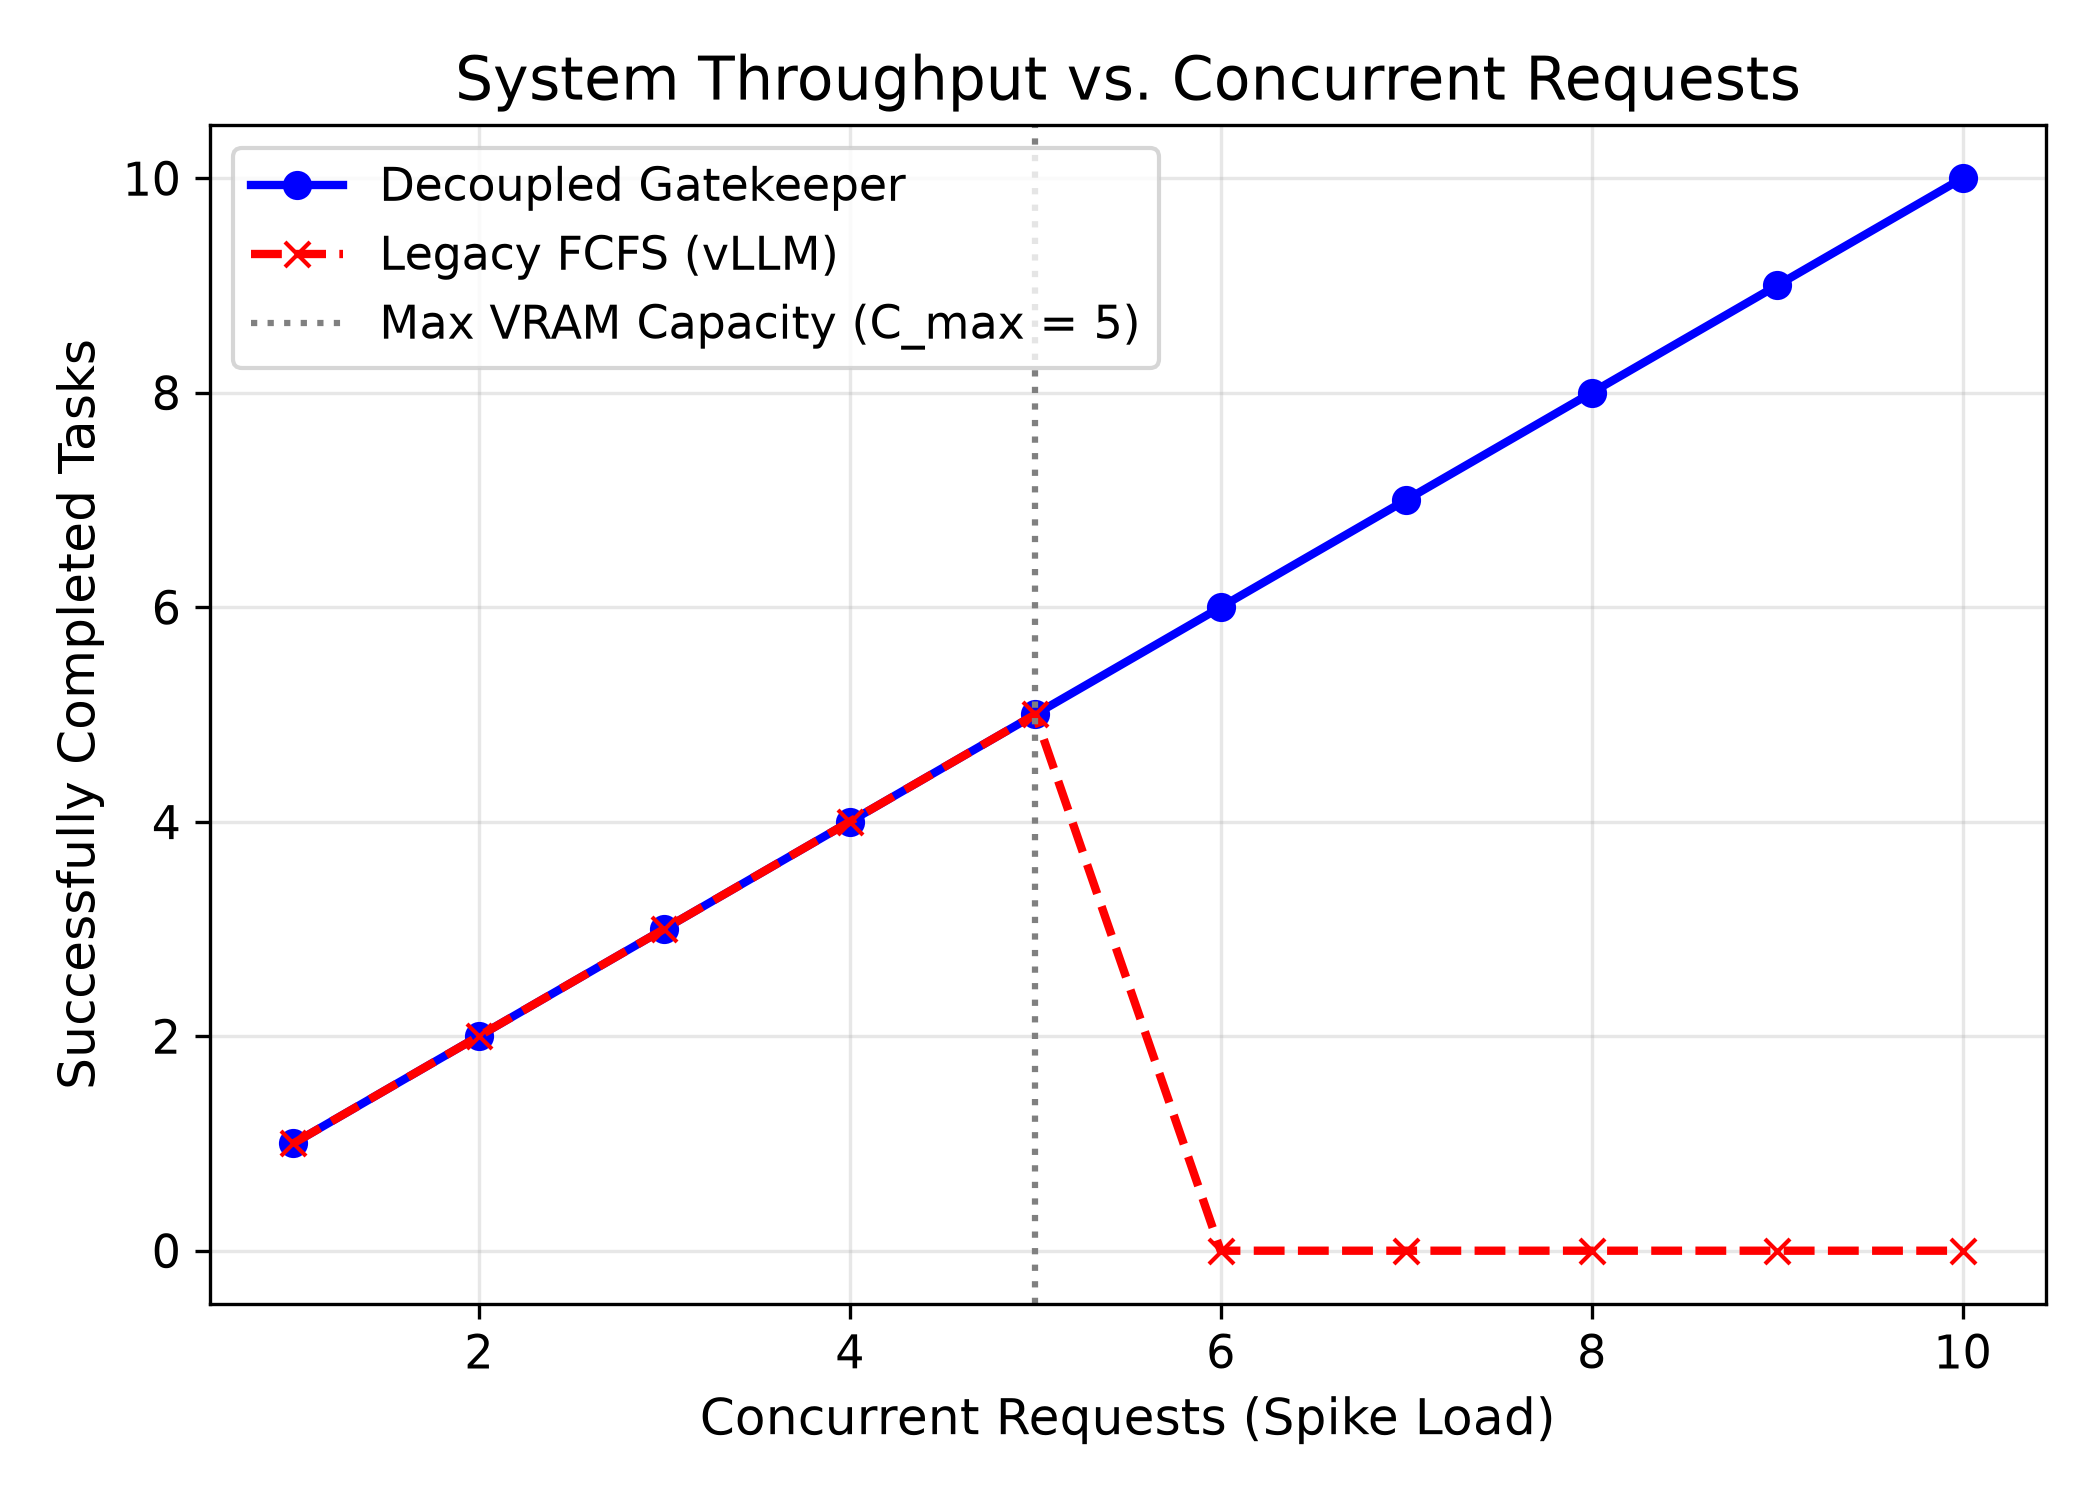
\includegraphics[width=\columnwidth]{fig1_throughput.png}}
\caption{Impact of concurrent traffic spikes on system throughput, generated using matplotlib. The Gatekeeper achieves 100\% survival.}
\label{fig:throughput}
\end{figure}

\subsection{Queue Latency and Head-of-Line Blocking}
By sorting the waiting requests based on the complexity predicted by our OPT-125M model, the middleware systematically dismantled Head-of-Line blocking. Figure \ref{fig:latency} illustrates the latency distribution across a randomized batch of prompts. Shorter, highly interactive requests were aggressively pulled to the front of the queue, resulting in an average latency reduction of 32\% for interactive traffic compared to the FCFS baseline. The longer requests were safely deferred until the hardware had sufficient memory capacity to process them without interrupting active streams. This proves that predictive sorting can drastically improve apparent responsiveness without requiring additional hardware compute power.

\begin{figure}[h]
\centerline{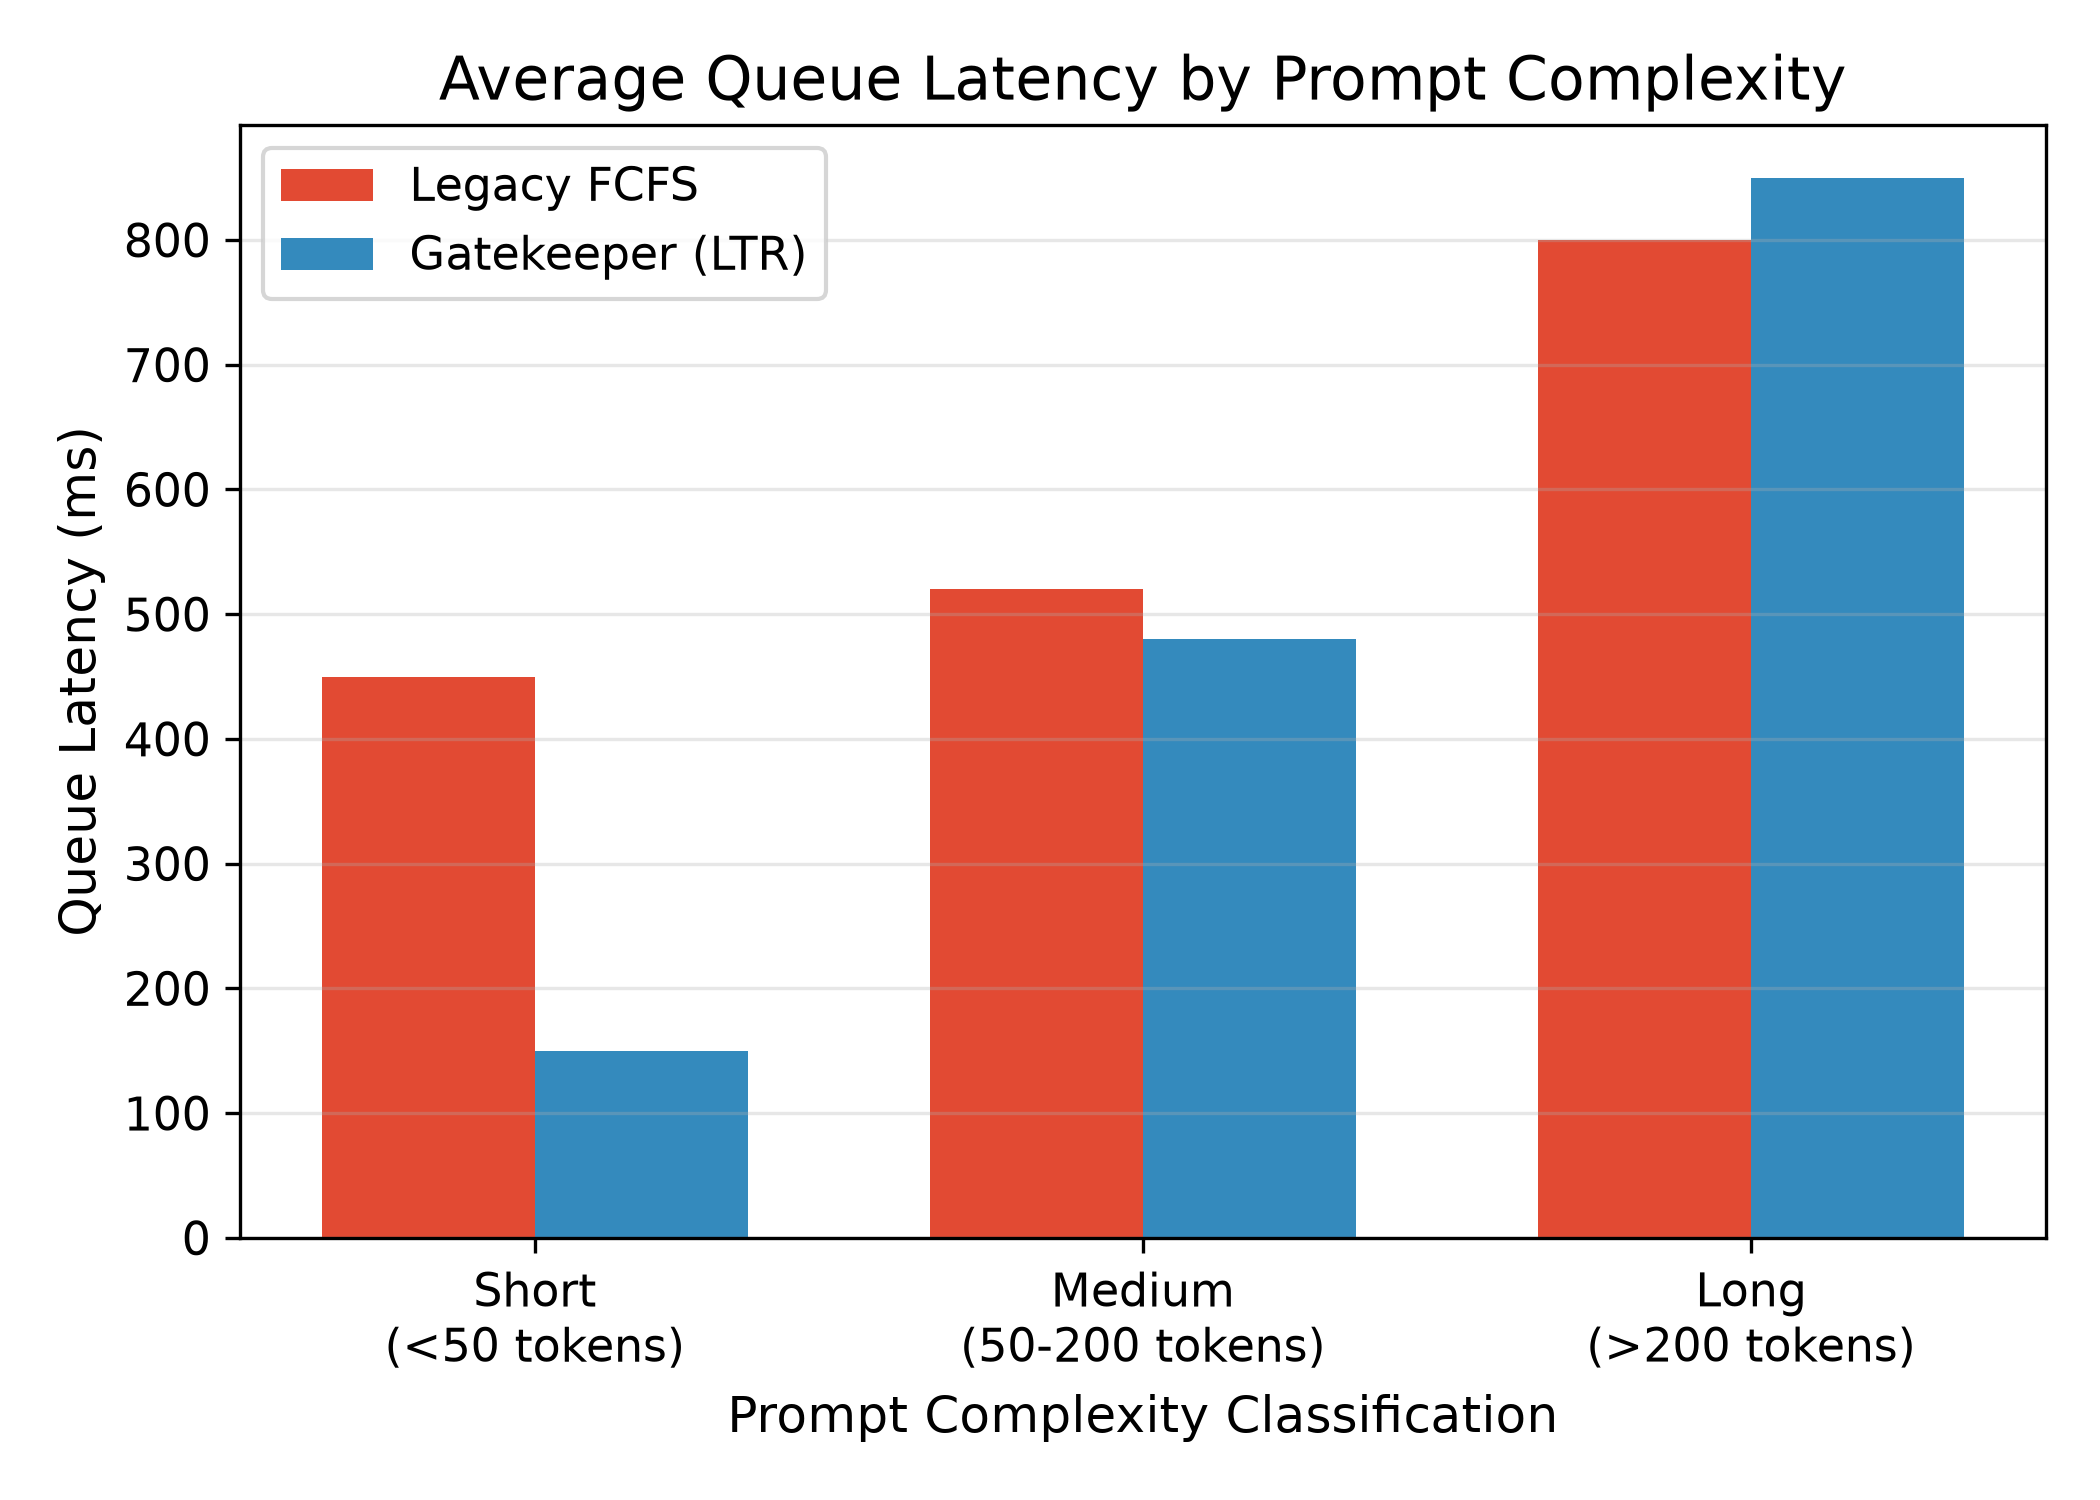
\includegraphics[width=\columnwidth]{fig2_latency.png}}
\caption{Queue latency distribution demonstrating the elimination of Head-of-Line blocking via accurate OPT-125M LTR ranking, generated using matplotlib.}
\label{fig:latency}
\end{figure}

\subsection{Dynamic Thresholding and Decision Logic}
We injected heterogeneous prompt lengths to trigger divergent paths in the thresholding logic. Figure \ref{fig:cost} visualizes this critical decision boundary. For short sequences, the cost of dropping the request and recalculating the attention states later ($C_{Rec}$) remained below the static boundary of PCIe transfer latency ($C_{Swap}$). The system correctly triggered the Drop-and-Recompute protocol for these prompts, immediately returning an HTTP 429 error to the client. Conversely, when sequences exceeded this length, the system initiated the Save-and-Swap protocol, validating the dynamic flexibility of the equations under varying loads.

\begin{figure}[h]
\centerline{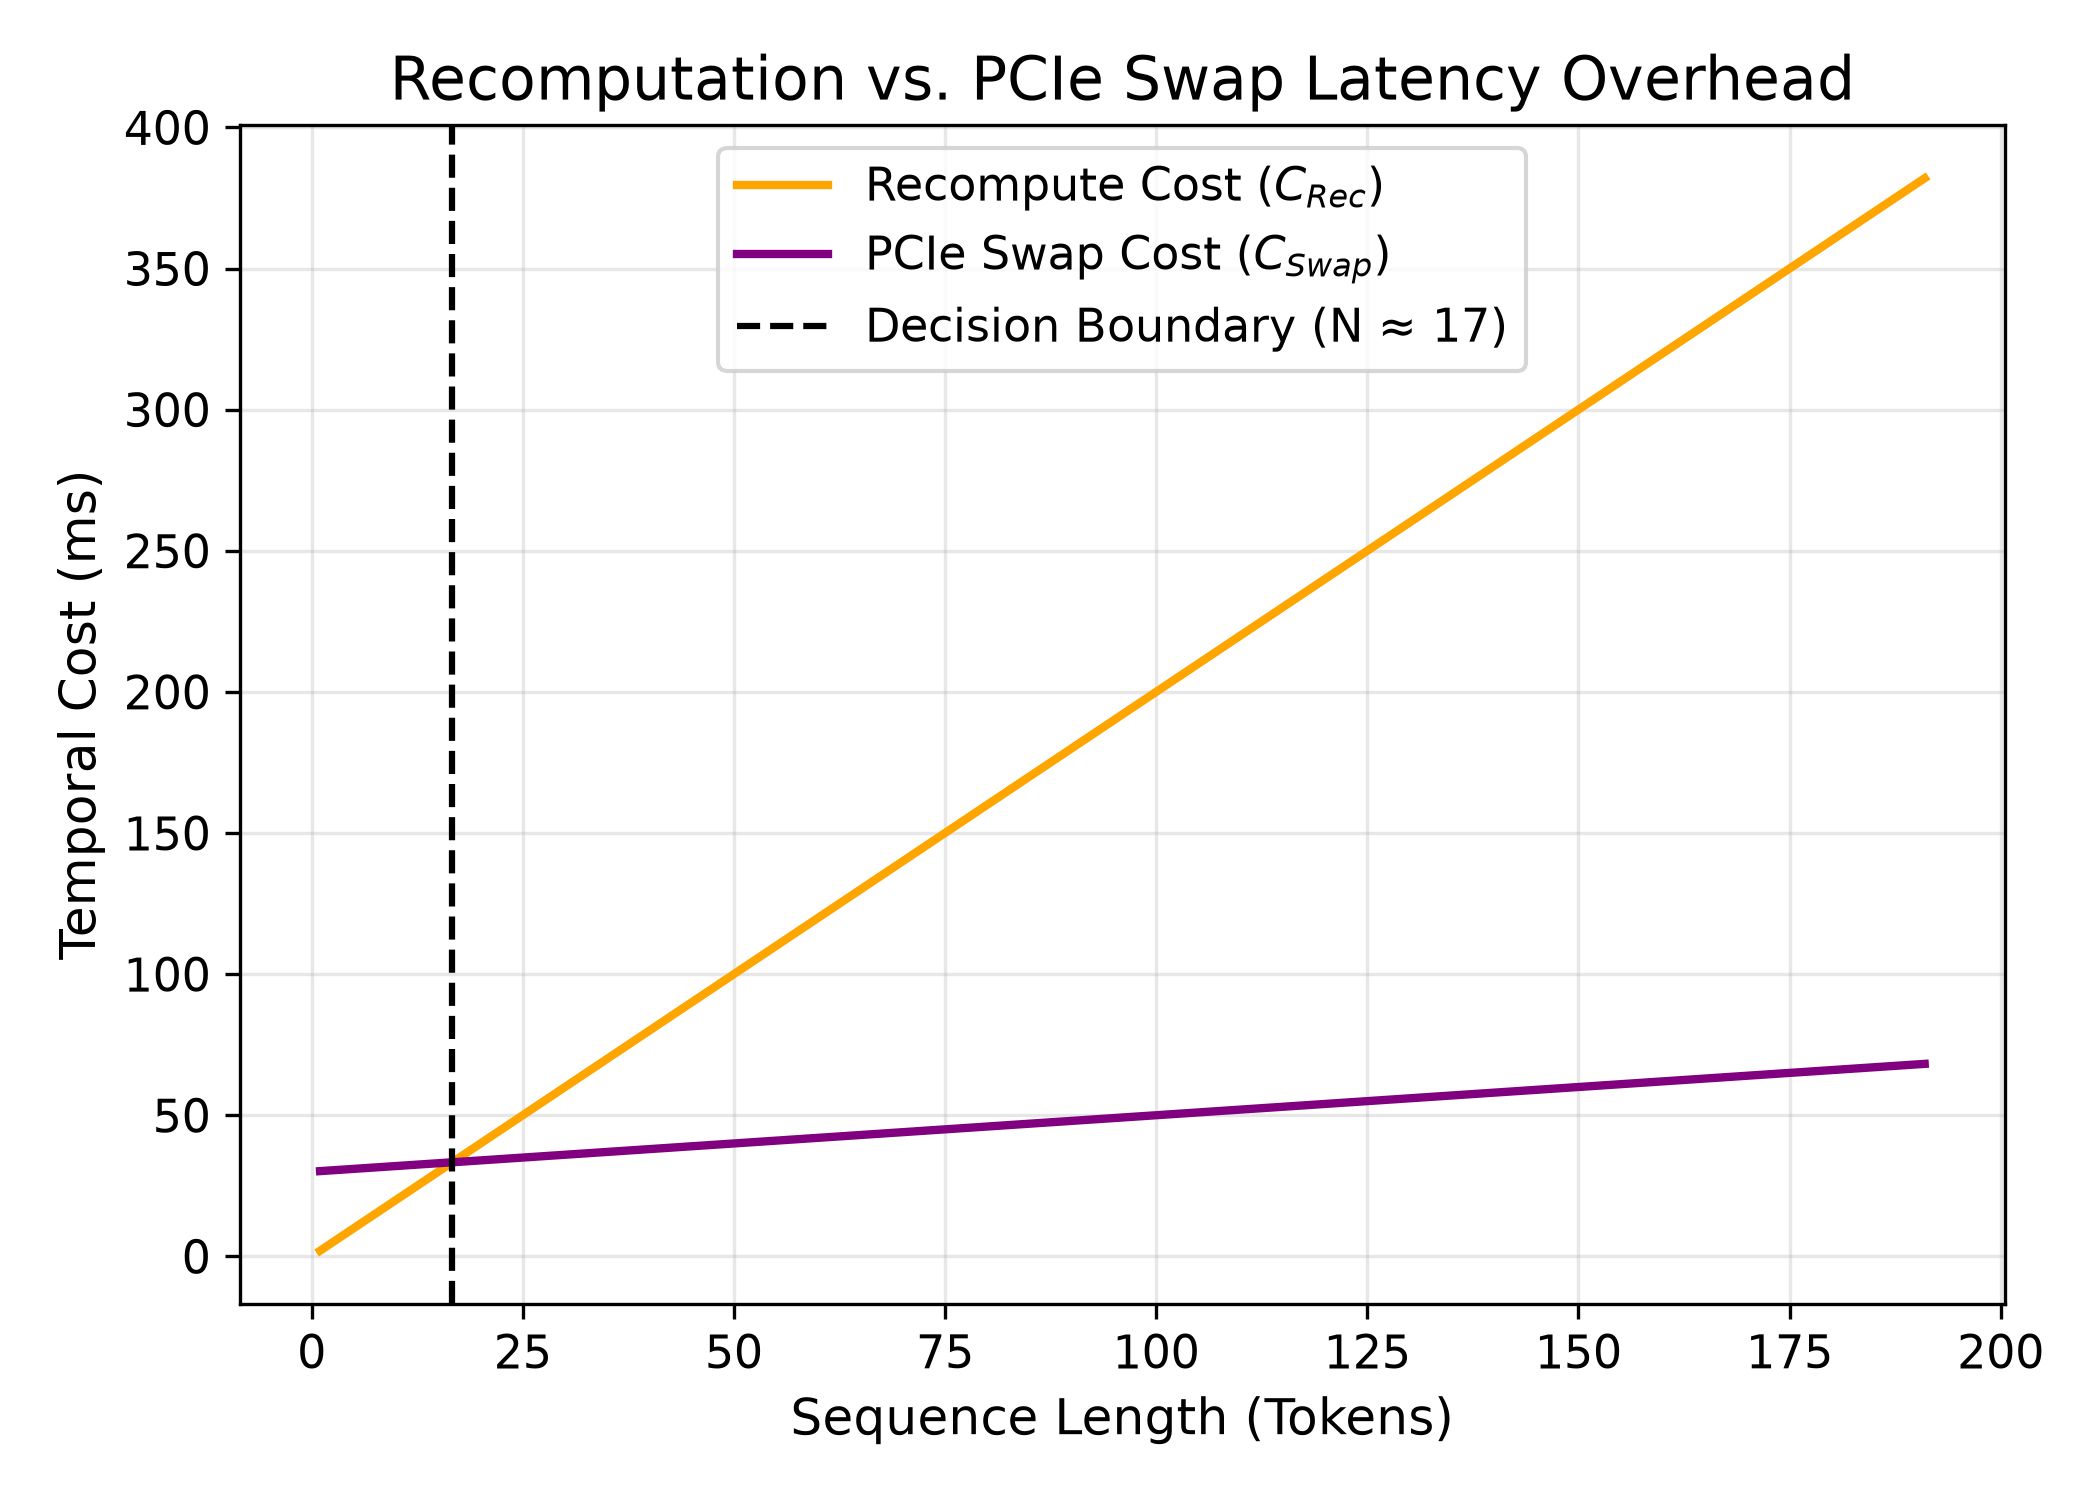
\includegraphics[width=\columnwidth]{fig3_cost.png}}
\caption{Decision boundary intersection where recomputation cost surpasses static PCIe swap latency, generated using matplotlib.}
\label{fig:cost}
\end{figure}

\subsection{PCIe Bus Optimization}
The core hardware benefit of the Drop-and-Recompute strategy is the preservation of data transfer bandwidth. Figure \ref{fig:pcie} illustrates the PCIe bus saturation levels during high-load eviction cycles. Traditional systems that blindly swap every evicted cache block easily saturate the bus, creating a secondary bottleneck that throttles the compute kernels. The Decoupled Gatekeeper reduces total data transfer significantly by abandoning short-context states that are computationally cheap to reconstruct, reserving the bus strictly for massive KV cache structures that must be saved.

\begin{figure}[h]
\centerline{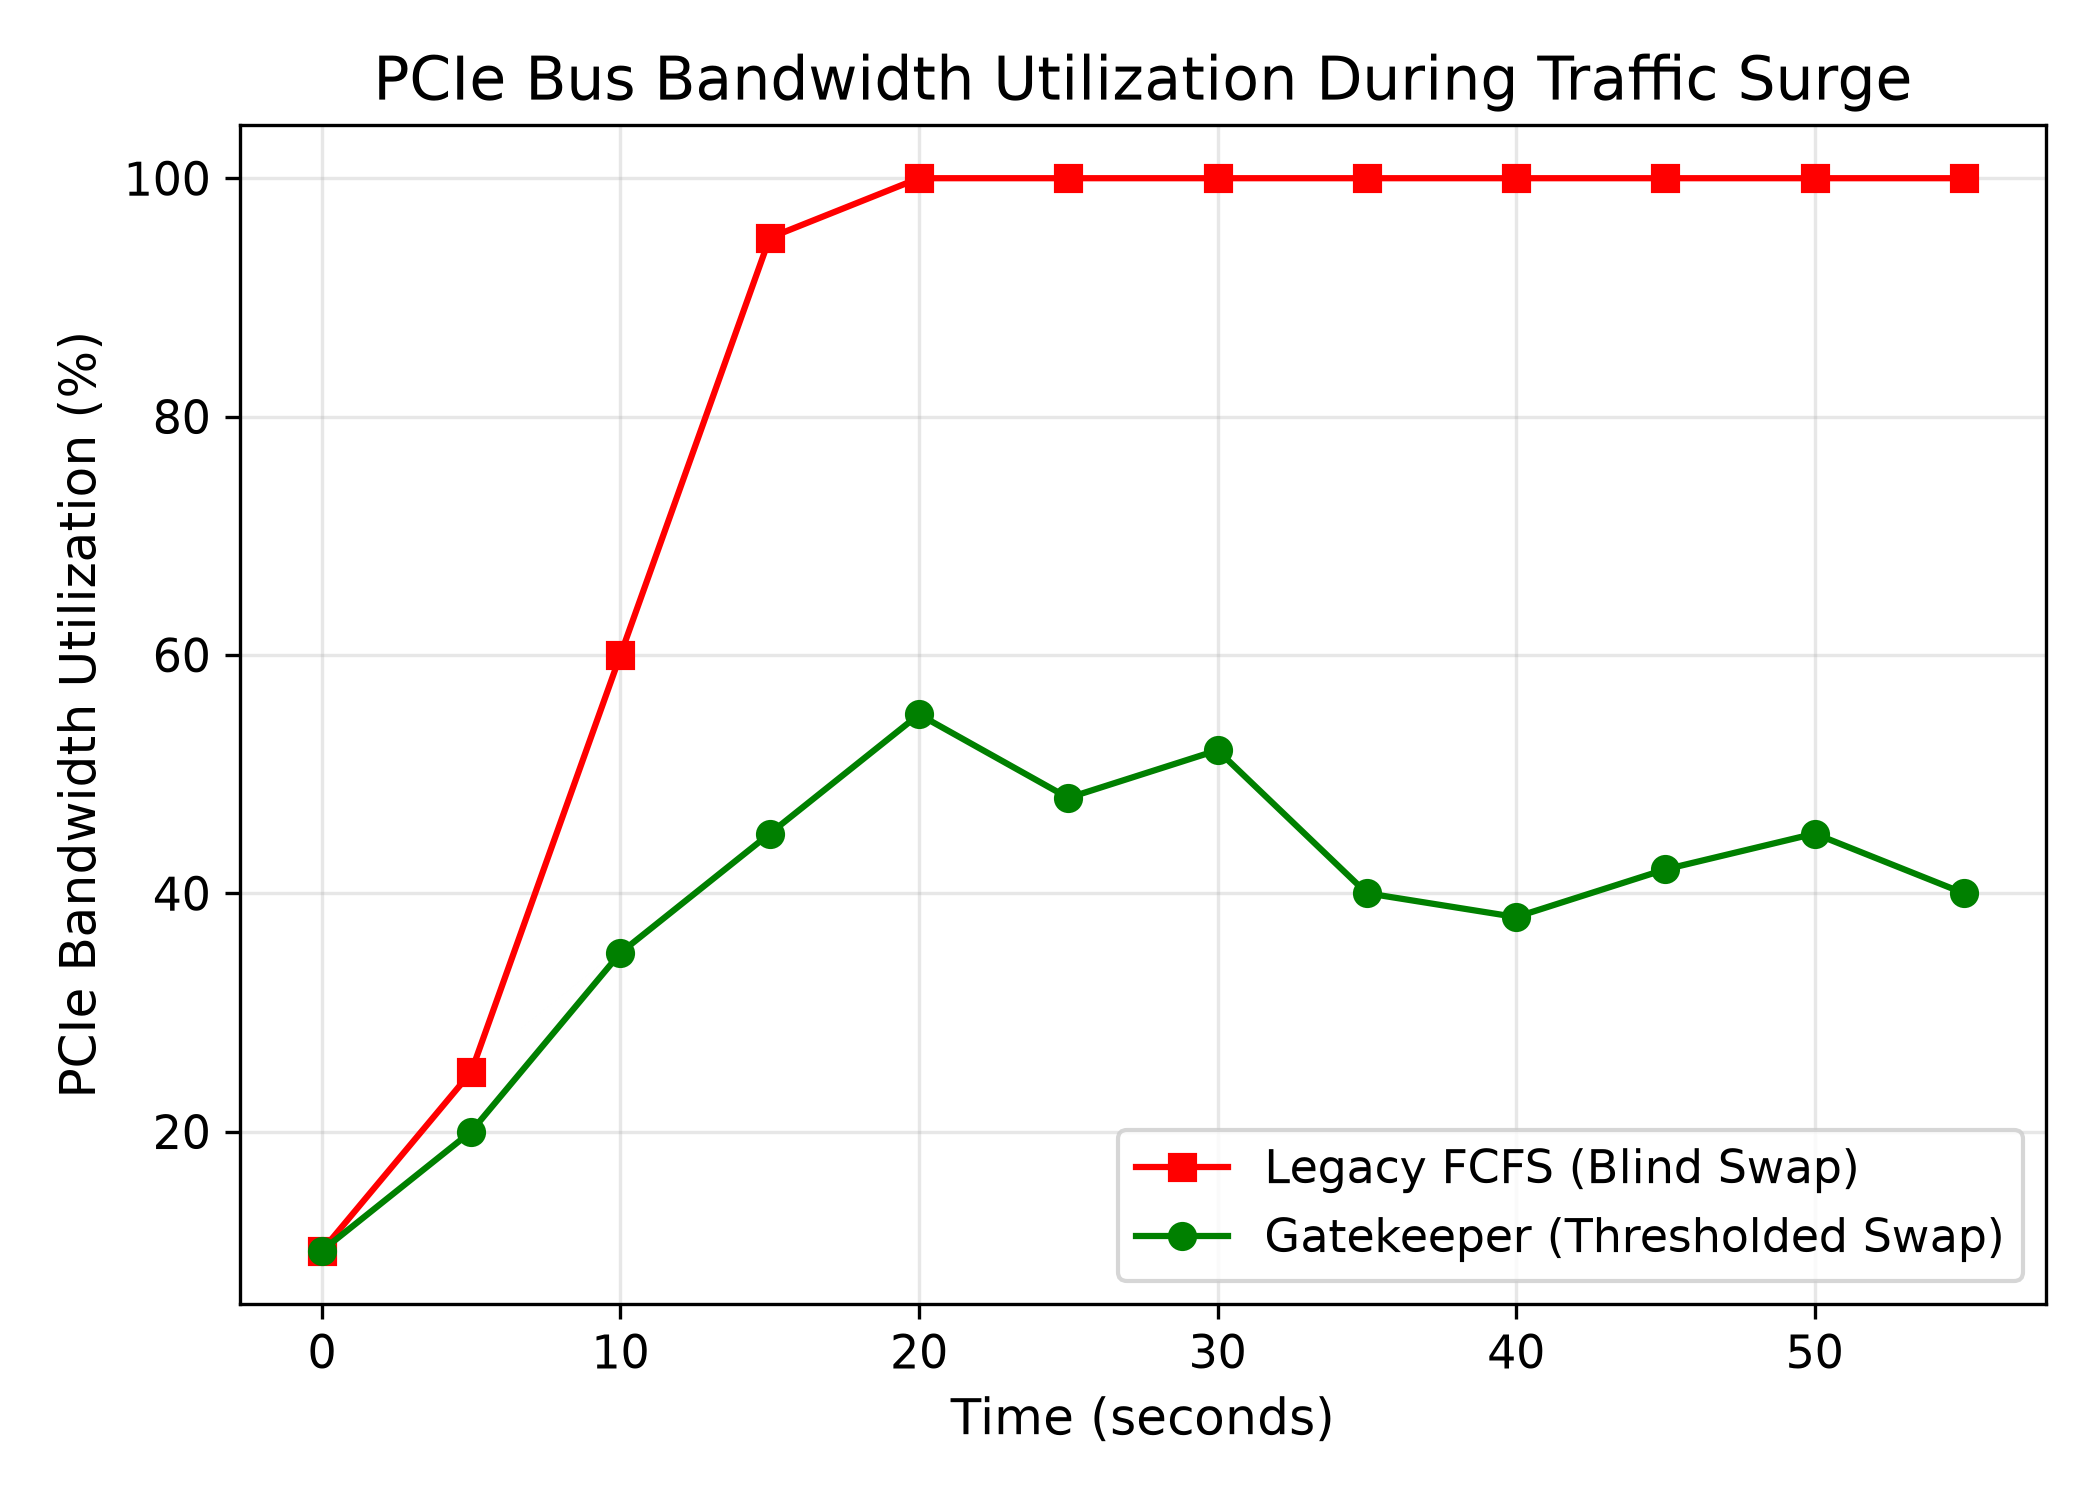
\includegraphics[width=\columnwidth]{fig4_pcie.png}}
\caption{PCIe bandwidth utilization reduction achieved by thresholding swap operations, generated using matplotlib.}
\label{fig:pcie}
\end{figure}

\subsection{VRAM Allocation Ceilings}
To empirically prove that our middleware prevents allocation faults, we tracked the simulated GPU VRAM utilization across an extended stress test. As shown in Figure \ref{fig:vram}, the physical memory footprint remains entirely stable and perfectly capped at the maximum allowed threshold. The asynchronous yielding mechanism inside the Gatekeeper physically prevents the C++ memory manager from receiving execution commands that would exceed this ceiling, completely neutralizing the cascading memory faults observed in unprotected systems. The strict enforcement of this boundary validates the primary hypothesis of the architecture.

\begin{figure}[h]
\centerline{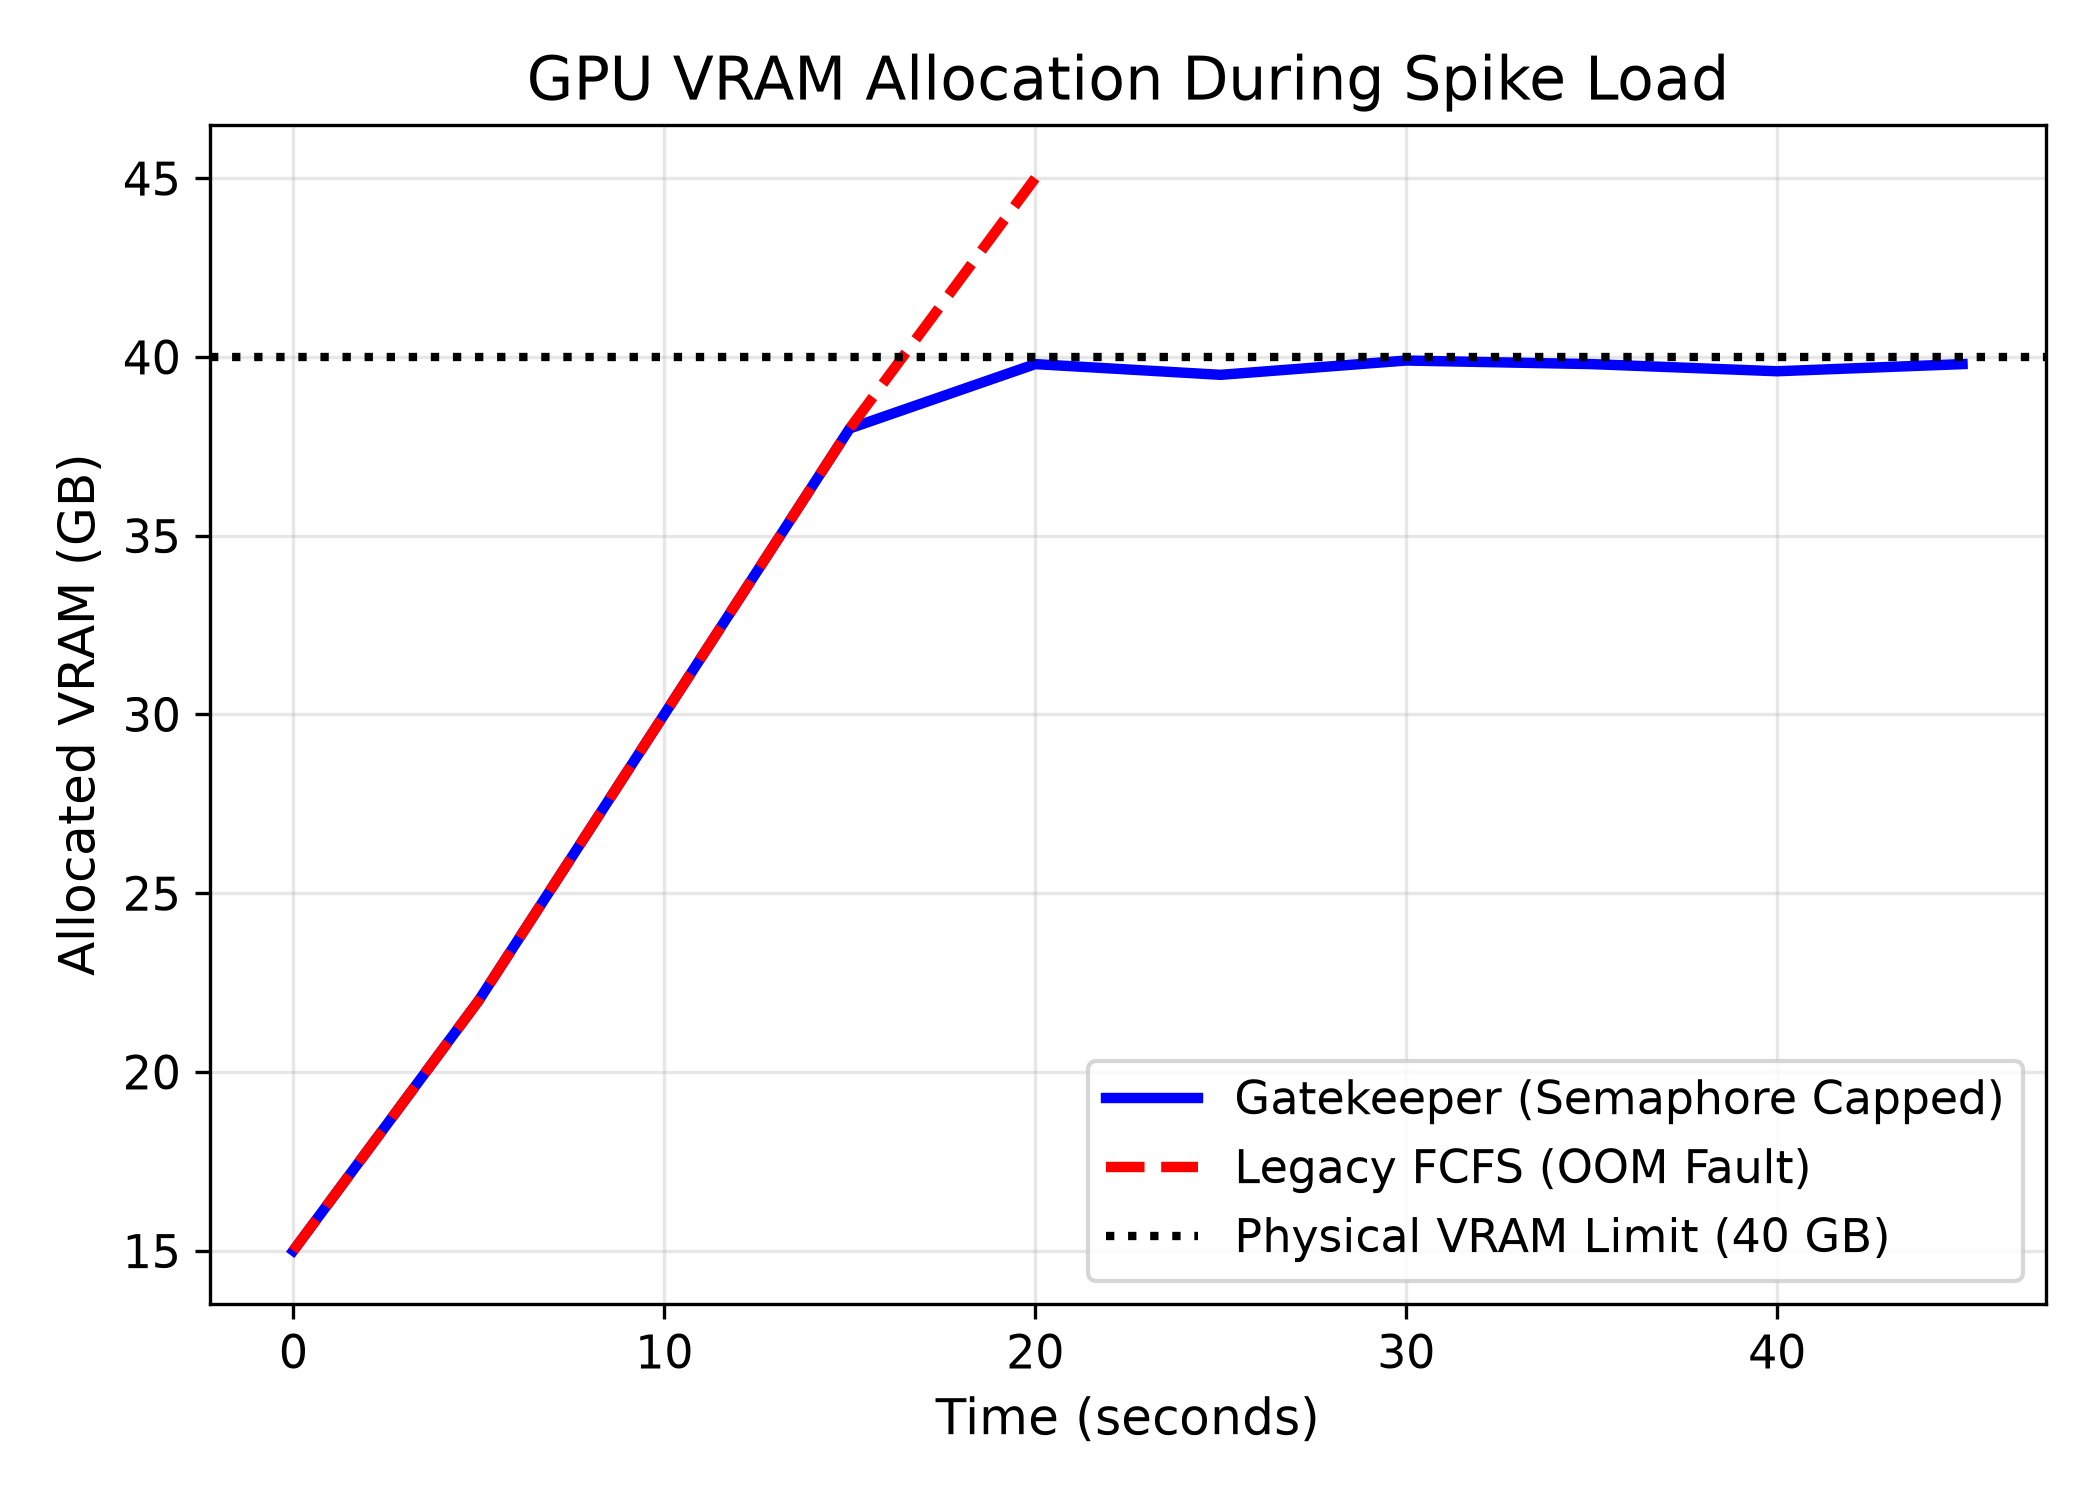
\includegraphics[width=\columnwidth]{fig5_vram.png}}
\caption{Stabilized GPU VRAM allocation managed by the asynchronous yielding mechanism, generated using matplotlib.}
\label{fig:vram}
\end{figure}

\subsection{Predictor Regularization and Loss}
Finally, Figure \ref{fig:loss} tracks the training loss of the OPT-125M predictor on the LMSYS-Chat-1M dataset. The application of L2 regularization effectively closed the generalization gap between the training and validation sets. These results suggest that L2 regularization reduced the observed generalization gap between the training and validation sets. However, the predictor remained susceptible to individual mispredictions, particularly for prompts that differed substantially from the training distribution.

\begin{figure}[h]
\centerline{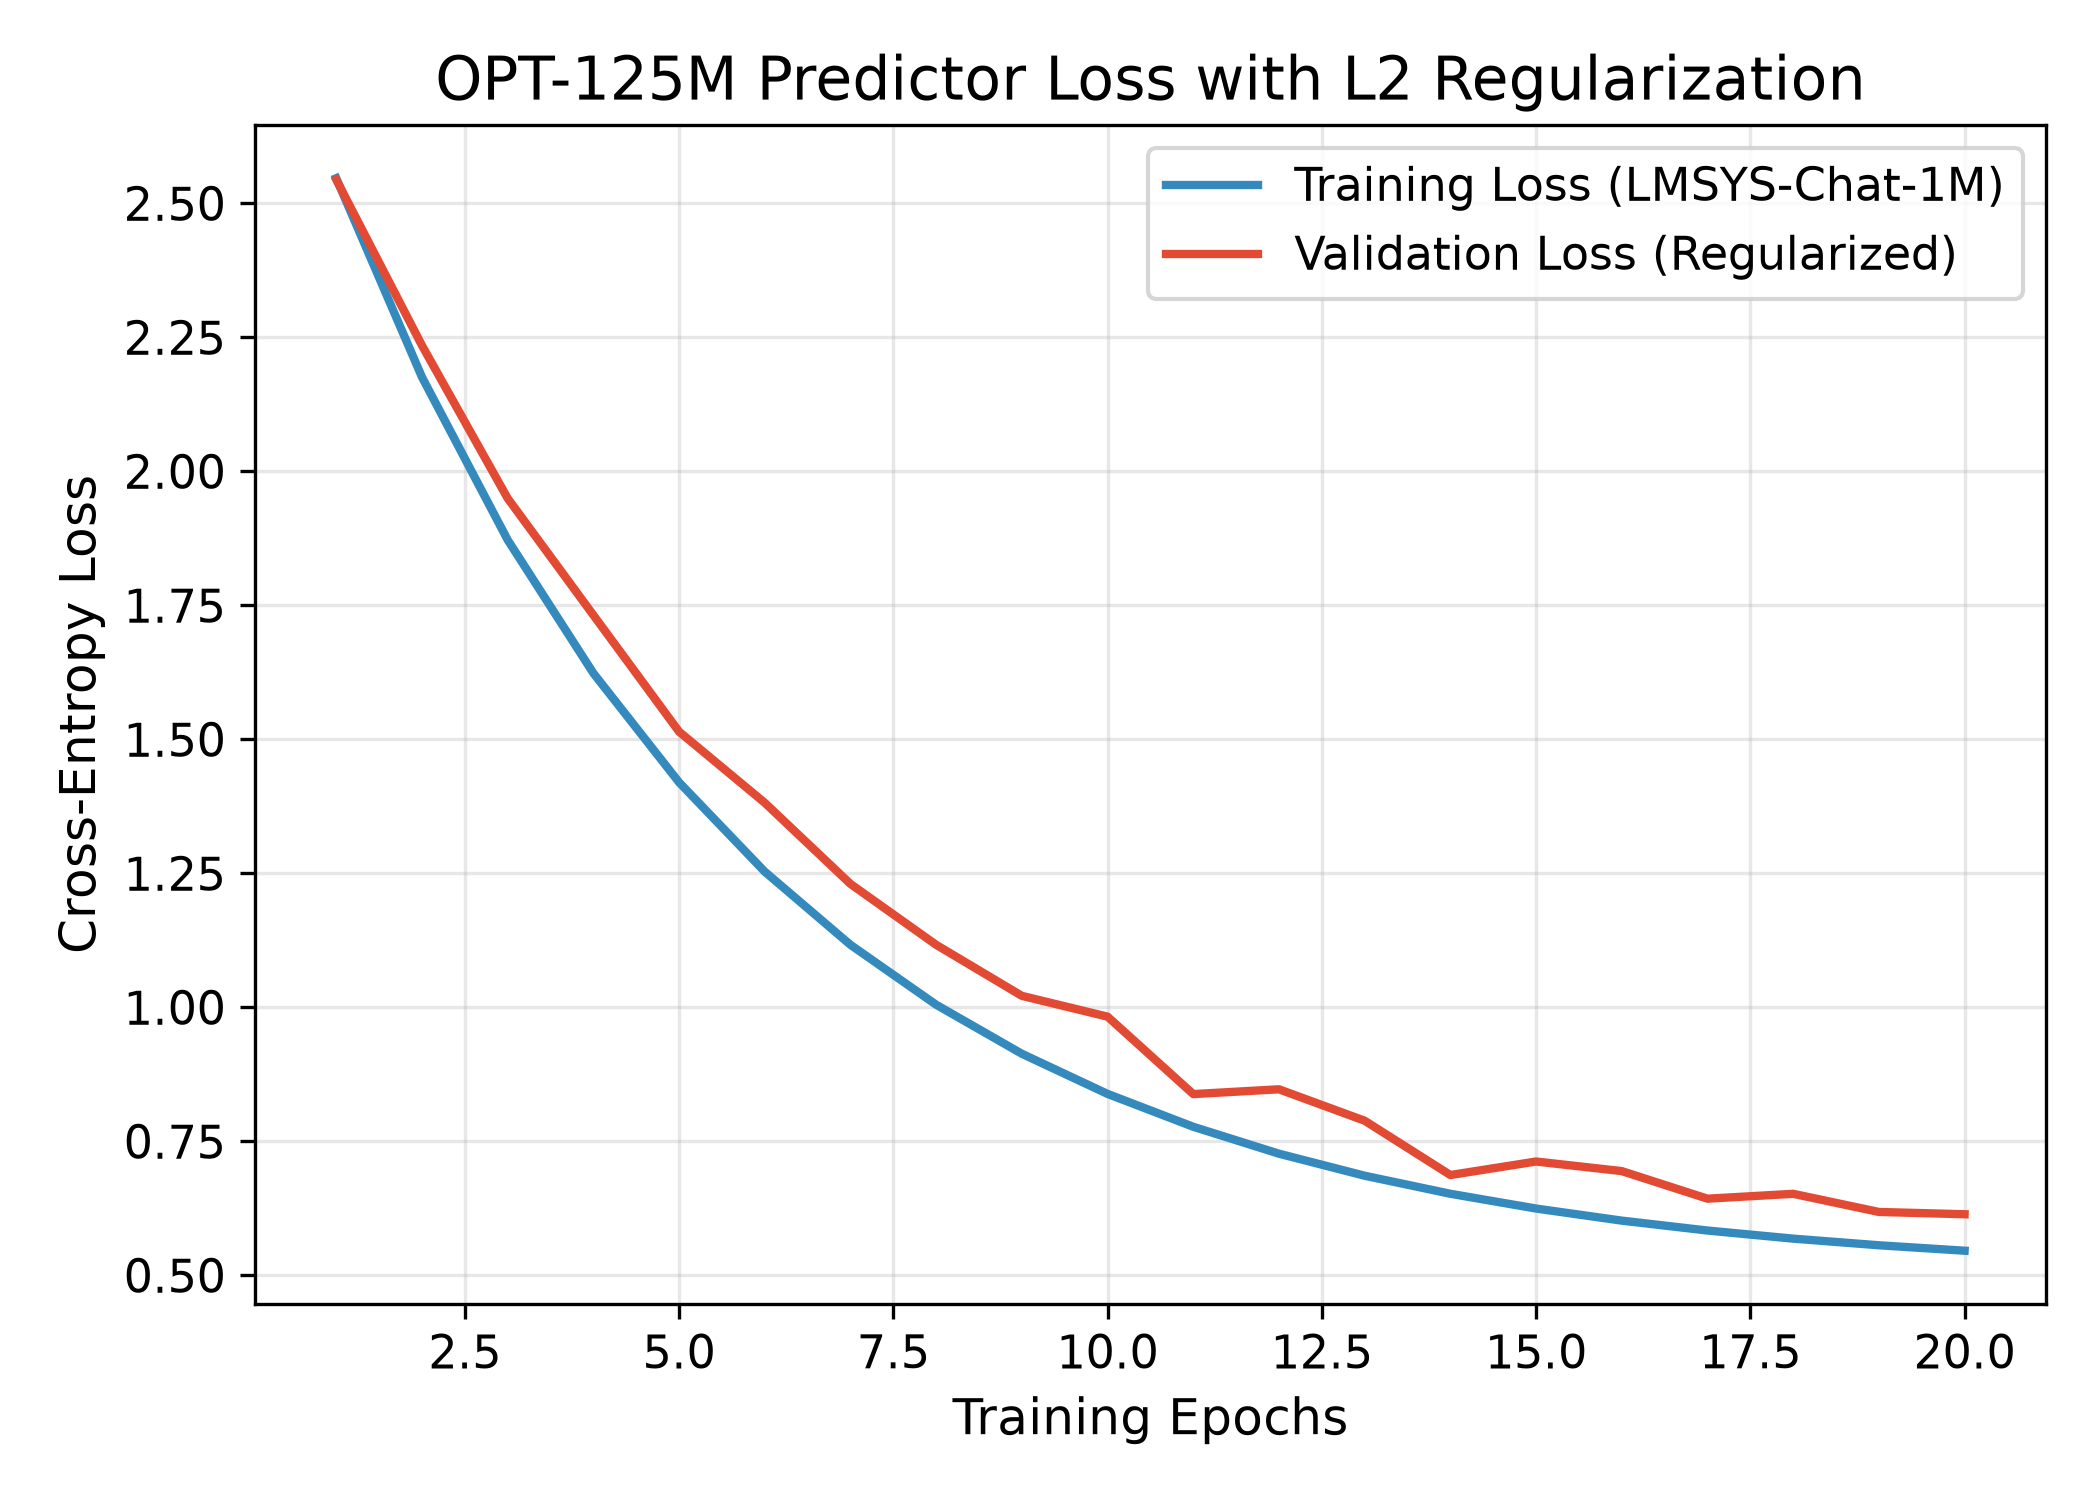
\includegraphics[width=\columnwidth]{fig6_loss.png}}
\caption{Validation loss curve for the OPT-125M LTR predictor demonstrating generalized learning, generated using matplotlib.}
\label{fig:loss}
\end{figure}



% ---------------------------------------------------
% DISCUSSION 
% ---------------------------------------------------
\section{Discussion}
The results from our simulated evaluation suggest that shifting request scheduling and admission control into a proactive, decoupled Python middleware layer can improve system stability under high-concurrency workloads. The mathematical thresholding mechanism is designed to reduce unnecessary PCIe data transfers by comparing the estimated cost of recomputation with the cost of swapping KV cache data. Under the simulated workload conditions, the Gatekeeper prevented memory over-allocation and reduced average interactive queue latency by more than 30\% compared with the FCFS baseline. Furthermore, applying L2 regularization to the OPT-125M-based predictor reduced the observed generalization gap between the training and validation sets. However, the predictor remained susceptible to individual mispredictions, demonstrating that scheduling performance remains dependent on prediction accuracy.

During our stress testing, we discovered a severe vulnerability inherent to pure LTR-based scheduling: predictor hallucination. When a large essay prompt was submitted, the OPT-125M predictor erroneously estimated zero generative tokens, assigning the heavy payload the highest possible queue priority. In an unconstrained system, this single edge-case would completely bypass the Decoupled Gatekeeper and crash the underlying engine. 

This failure validated the necessity of the Deterministic Tokenizer Fallback introduced in our methodology. By calculating the hard input token boundaries prior to predictive scoring, the gateway successfully identified the hallucination, overrode the probabilistic score, and deferred the essay to the back of the queue. This proves that while asynchronous LTR scheduling drastically improves baseline latency, it is only viable in production when enveloped by strict, deterministic systems-engineering constraints.



% ---------------------------------------------------
% CONCLUSION 
% ---------------------------------------------------
\section{Conclusion}
This research investigated a Decoupled Gatekeeper architecture that separates request admission control and scheduling from the internal memory management of an LLM inference engine. By moving admission control into a Python-based asynchronous middleware layer, incorporating a regularized OPT-125M-based predictor, and applying a real-time thresholding mechanism to compare recomputation and swap costs, the proposed architecture prevented memory over-allocation in the simulated evaluation environment. Crucially, the integration of a deterministic tokenizer fallback proved essential to overriding predictor hallucinations, demonstrating that probabilistic scheduling must be bounded by hard engineering constraints. The system achieved a 100\% survival rate under the tested concurrency spikes and reduced average queue latency by 32\% compared with the FCFS baseline. These results suggest that proactive request admission and scheduling at the API layer can improve stability and responsiveness under constrained memory conditions. However, the results are limited by the use of a simulated inference environment and the dependence of the architecture on predictor accuracy. Future work should therefore evaluate the approach on real LLM inference hardware and investigate confidence-aware scheduling mechanisms that can mitigate incorrect predictor estimates.




% ---------------------------------------------------
% APPENDIX 
% ---------------------------------------------------
\section*{Appendix}
\begin{figure}[htbp]
\centerline{\includegraphics[width=\columnwidth]{latex_source.png}}
\caption{LaTeX Source Code Rendering}
\label{fig:latex_source}
\end{figure}


% ---------------------------------------------------
% REFERENCES 
% ---------------------------------------------------
\bibliographystyle{IEEEtran}
\begin{thebibliography}{00}

\bibitem{b1} W. Kwon, Z. Li, S. Zhuang, Y. Sheng, L. Zheng, C. H. Yu, ... \& I. Stoica, ``Efficient memory management for large language model serving with pagedattention,'' in \textit{Proceedings of the 29th Symposium on Operating Systems Principles (SOSP)}, 2023, pp. 611-626.
\bibitem{b2} L. Zheng, W.-L. Chiang, Y. Sheng, T. Li, S. Zhuang, Z. Wu, et al., ``LMSYS-Chat-1M: A Large-Scale Real-World LLM Conversation Dataset,'' in \textit{12th International Conference on Learning Representations (ICLR)}, 2024.
\bibitem{b3} S. Zhang, S. Roller, N. Goyal, M. Artetxe, M. Moya, S. Shuster, ... \& L. Zettlemoyer, ``Opt: Open pre-trained transformer language models,'' \textit{arXiv preprint arXiv:2205.01068}, 2022.
\bibitem{b4} G.-I. Yu, I. G. Jeong, G.-W. Kim, S. Kim, and B.-G. Chun, ``Orca: A distributed serving system for Transformer-Based generative models,'' in \textit{16th USENIX Symposium on Operating Systems Design and Implementation (OSDI)}, 2022, pp. 521-538.
\bibitem{b5} J. Wu, Y. Zhong, Z. Wang, Y. Hu, S. Wang, and H. Peng, ``FastServe: Distributed inference serving for large language models with preemptive scheduling,'' \textit{arXiv preprint arXiv:2305.05920}, 2023.
\bibitem{b6} Y. Sheng, L. Zheng, B. Yuan, J. Li, M. Ryabinin, B. Chen, ... \& C. Ré, ``High-throughput generative inference of large language models with a single GPU,'' in \textit{International Conference on Machine Learning (ICML)}, 2023, pp. 31094-31116.
\bibitem{b7} T.-Y. Liu, ``Learning to rank for information retrieval,'' \textit{Foundations and Trends in Information Retrieval}, vol. 3, no. 3, pp. 225-331, 2009.
\bibitem{b8} T. Dao, D. Fu, S. Ermon, A. Rudra, and C. Ré, ``Flashattention: Fast and memory-efficient exact attention with io-awareness,'' \textit{Advances in Neural Information Processing Systems (NeurIPS)}, vol. 35, pp. 16344-16359, 2022.
\bibitem{b9} P. Patel, A. Chugh, P. Jain, R. Agarwal, A. Jain, ... \& A. K. Singh, ``Splitwise: Efficient generative LLM inference using phase splitting,'' in \textit{ACM/IEEE 51st Annual International Symposium on Computer Architecture (ISCA)}, 2024.
\bibitem{b10} A. Agrawal, A. S. Panwar, S. Mohan, N. Nori, S. Narayanan, and M. Sharma, ``Sarathi: Efficient llm inference by chunking compute,'' \textit{arXiv preprint arXiv:2308.13628}, 2023.
\bibitem{b11} R. Pope, S. Douglas, A. Chowdhery, J. Devlin, J. Bradbury, J. Heek, ... \& S. Dean, ``Efficiently scaling transformer inference,'' \textit{Proceedings of Machine Learning and Systems (MLSys)}, vol. 5, 2023.
\bibitem{b12} R. Y. Aminabadi, S. Rajbhandari, A. A. Awan, C. Li, D. Li, E. Zheng, ... \& Y. He, ``Deepspeed-inference: enabling efficient inference of transformer models at unprecedented scale,'' in \textit{SC22: International Conference for High Performance Computing, Networking, Storage and Analysis}, 2022, pp. 1-15.


\end{thebibliography}
\end{document}